\chapter{Dropbox}\label{chap:dropbox}

\section{Motivation and Background}
Dropbox was born out of a simple yet pervasive frustration: the hassle of accessing files on multiple devices. The idea took shape when co-founder Drew Houston repeatedly forgot his USB drive—a common inconvenience that highlighted a broader need for seamless file synchronization and remote access \cite{BusinessInsider2018}.

Inspired in part by the efficient file access model of MIT’s Athena system, which enabled students to retrieve files from any campus workstation, Houston envisioned a system that brought similar convenience to the general public. Thus, Dropbox emerged as an innovative cloud storage solution aimed at eliminating the dependency on physical storage devices \cite{Awfis2021}.

\section{Key Problems Addressed}
\subsection{Challenges Before Dropbox}
\begin{itemize}
    \item \textbf{Reliance on Physical Storage:} Users had to carry USB drives or email files to themselves, which was not only inconvenient but also prone to loss or damage.
    \item \textbf{File Versioning Issues:} Maintaining the latest version of a file across various devices, especially during collaborations, was a persistent challenge.
    \item \textbf{Unreliable Existing Tools:} Early file-syncing tools were often buggy, slow, and required extensive manual configuration.
    \item \textbf{Limited Remote Access:} Accessing files from remote locations typically involved cumbersome methods, reducing overall productivity.
\end{itemize}

\subsection{Dropbox's Innovative Solutions}
\begin{itemize}
    \item \textbf{Automatic File Synchronization:} Files are updated in real time across all connected devices, ensuring users always work with the latest version.
    \item \textbf{Cloud Storage Infrastructure:} By storing files remotely, Dropbox minimizes the risk of data loss from hardware failures.
    \item \textbf{Robust Version Control:} Users can effortlessly recover previous versions of their files, which is invaluable during collaborative projects.
    \item \textbf{User-Friendly Interface:} An intuitive drag-and-drop functionality makes file management simple and integrates seamlessly with existing file systems.
    \item \textbf{Enhanced Collaboration:} Shared folders and real-time updates foster smoother teamwork, eliminating the need for repetitive file transfers.
\end{itemize}


\section{Challenges}
Dropbox-like systems face several unique challenges that stem from their core mission to provide seamless, efficient, and secure file synchronization across a variety of devices. Some of these challenges include:

\begin{enumerate}
    \item \textbf{High Read-to-Write Ratio (~1:1):} With continuous synchronization across multiple devices, Dropbox experiences nearly as many reads as writes, necessitating efficient caching and deduplication mechanisms 
    \item \textbf{Conflict Resolution in Synchronization:} Efficiently managing version conflicts when multiple users edit the same file is crucial to prevent data loss and ensure a smooth user experience 
    \item \textbf{Efficient Metadata Storage:} With millions of files per user, optimizing metadata storage and retrieval is vital for maintaining performance.
    \item \textbf{Eventual Consistency vs. Strong Consistency:} To ensure smooth synchronization, Dropbox prioritizes eventual consistency, which may lead to temporary file discrepancies 
    \item \textbf{Efficient Data Deduplication:} Storing only one copy of identical files or blocks helps reduce storage costs and improves system efficiency 
    \item \textbf{Bandwidth Optimization:} Techniques such as compression, differential synchronization, and intelligent throttling are used to minimize network usage during file transfers 
    \item \textbf{Handling Offline Changes:} Detecting edits made while offline and synchronizing them accurately when the device reconnects presents unique challenges.
    \item \textbf{Delta Encoding for Efficient Transfers:} Transmitting only the byte-level differences between file versions rather than full file copies is critical for reducing data transfer volumes 
    \item \textbf{Multi-Device Conflict Handling at Scale:} Employing timestamp-based versioning and user notifications helps resolve conflicts that arise from simultaneous edits on multiple devices.
    \item \textbf{Global Namespace Management:} Preventing file path collisions and ensuring fast lookup in a distributed system is essential for maintaining a consistent user experience 
    \item \textbf{Latency Reduction in Large Folder Syncs:} Prioritizing critical files while indexing large directories in the background minimizes perceived latency during synchronization 
\end{enumerate}


\section{Architecture}
Dropbox's system architecture has evolved from a simple file synchronization model to a distributed, highly scalable, and fault-tolerant platform. This section details the evolution and technical design of both server- and client-side components.

\subsection{Initial Design}
The early architecture was based on a straightforward client-server model:
\begin{itemize}
    \item \textbf{Client Application:} Monitors local file changes and communicates with the server.
    \item \textbf{Central Server:} Stores files and manages metadata.
    \item \textbf{Full-file Synchronization:} Entire files were transmitted for each update, leading to inefficient bandwidth and storage use.
\end{itemize}

\subsection{Enhanced Server Architecture}
To meet increased demands, the backend was re-engineered into modular components, as illustrated in \Cref{fig:write-path}.

\begin{figure}[H]
    \centering
    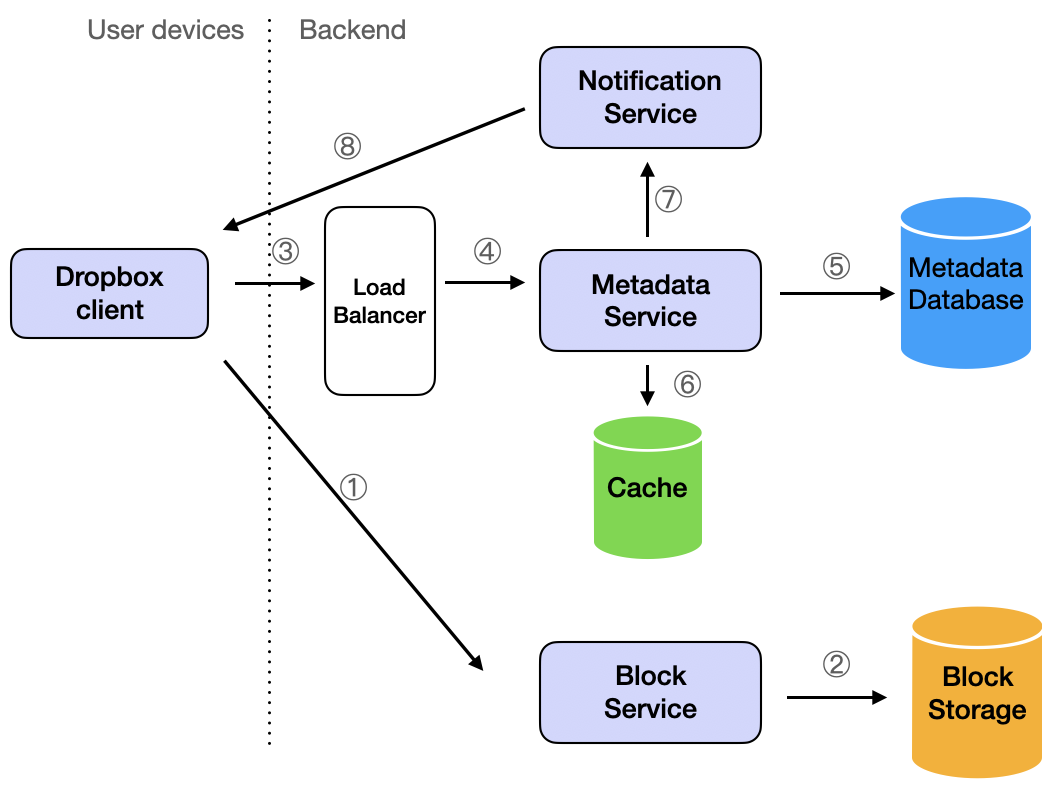
\includegraphics[width=0.8\textwidth]{img/write-path.png}
    \caption{Server-side Architecture: The Metadata Service uses a key-value store; the Block Service manages file chunks in a distributed file system; the Notification Service propagates updates; and the Load Balancer distributes client requests efficiently[Source: \cite{Dropbox_solution2}].}
    \label{fig:write-path}
\end{figure}

\subsubsection{File Chunking and Deduplication}
Files are partitioned into fixed-size 4MB chunks. Each chunk is processed with a cryptographic hash (SHA-256) to:
\begin{itemize}
    \item Uniquely identify the data block.
    \item Verify data integrity.
    \item Enable deduplication by referencing existing chunks when identical data is encountered.
\end{itemize}

\subsubsection{Block Server}
The Block Server employs a key-value storage paradigm where each SHA-256 hash acts as the key for its corresponding chunk. This design allows for rapid retrieval and minimizes redundant storage.

\subsubsection{Metadata Management}
Metadata—including file paths, versioning, and offsets—is stored in a hierarchical key-value database (e.g., LevelDB). The Metadata Service:
\begin{itemize}
    \item Synchronizes file metadata between clients and the server.
    \item Computes and disseminates incremental change sets.
    \item Interfaces with the Notification Service to propagate updates in real time.
\end{itemize}

\subsubsection{Notification Service}
A dedicated Notification Service broadcasts file update events to all subscribed clients, ensuring low-latency synchronization across devices.

\subsubsection{Load Balancing and Inter-Service Communication}
A round-robin load balancer distributes incoming requests evenly across metadata servers. Asynchronous message queues are employed to facilitate non-blocking communication between services, thereby enhancing scalability and resilience.

\subsection{Client Architecture}
Client-side improvements focus on efficient file handling and robust synchronization. \Cref{fig:client} shows the refined client workflow.

\begin{figure}[H]
    \centering
    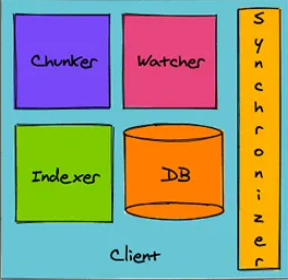
\includegraphics[width=0.4\textwidth]{img/client.png}
    \caption{Client Architecture: Integrates a file chunker, Metadata Service client, file watcher, local metadata indexer, and a synchronizer that coordinates with remote services [Source: \cite{Dropbox_solution1}].}
    \label{fig:client}
\end{figure}

\begin{enumerate}
    \item \textbf{Chunker:} Segments files into 4MB blocks for efficient block-level transmission.
    \item \textbf{Metadata Service Client:} Handles bidirectional communication with the Metadata Service to exchange change sets.
    \item \textbf{File Watcher:} Monitors local file system events and triggers indexing updates.
    \item \textbf{Indexer:} Updates the local metadata repository and notifies the synchronizer upon detecting changes.
    \item \textbf{Synchronizer:} Reconciles local state with remote services by coordinating metadata and block updates, handling both push and pull synchronization modes.
\end{enumerate}


\section{Optimizations over the Naive Approach}

\subsection{Efficient File Synchronization via DeltaSync}

DeltaSync minimizes data transfer by employing advanced delta encoding techniques that target only the modified portions of files. Its design philosophy is to reduce bandwidth usage, avoid redundant transmissions, and achieve near-real-time updates.

\subsubsection{Rolling Hash-based Content Defined Chunking (CDC)}
To overcome the limitations of fixed-size chunking (the \emph{block shift problem}), DeltaSync uses a rolling hash function to determine chunk boundaries based on file content:
\begin{enumerate}
    \item \textbf{Block Hashing:} The file is processed with a sliding window to compute a rolling hash for each tentative block.
    \item \textbf{Dynamic Boundary Detection:} A chunk boundary is defined when the hash satisfies:
    \[
        H_i \mod T = 0,
    \]
    where \(H_i\) is the current hash and \(T\) is a threshold parameter set to achieve an optimal average chunk size.
    \item \textbf{Efficient Update Mechanism:} The rolling hash is updated as:
    \[
        H_i = \Bigl( H_{i-1} - B_{i-1} \cdot P^{w-1} \Bigr) \cdot P + B_{i+w-1} \mod M,
    \]
    with:
    \begin{itemize}
        \item \(B_{i-1}\) and \(B_{i+w-1}\) as the outgoing and incoming bytes,
        \item \(P\) as a prime number,
        \item \(w\) as the window size,
        \item \(M\) as a modulus.
    \end{itemize}
\end{enumerate}

\subsubsection{Handling Insertions and Deletions}
By leveraging CDC, DeltaSync re-aligns chunk boundaries dynamically. For example:
\[
\text{Original: } [A][B][C][D][E] \quad \Longrightarrow \quad \text{Modified: } [A][B'] [X] [C][D][E],
\]
where only the affected chunks (\(B'\) and \(X\)) require retransmission.

\subsubsection{Supplementary Optimizations}
Additional technical enhancements include:
\begin{itemize}
    \item \textbf{Deduplication:} Transmitting and storing only unique chunks across files and users.
    \item \textbf{Compression:} Compressing data to further reduce transmission size.
    \item \textbf{Parallel Transfers:} Uploading multiple modified chunks concurrently to maximize throughput.
\end{itemize}

\subsection{Real-Time Notifications via Long Polling}

Long polling is employed to notify clients of file changes in near real-time while maintaining minimal resource overhead. Its core philosophy is to balance immediacy with scalability.

\subsubsection{Mechanism Overview}

Long polling maintains an open HTTP connection until a file event occurs:
\begin{enumerate}
    \item \textbf{Initiate Request:}
    \begin{lstlisting}
GET https://notify.dropboxapi.com/2/files/list_folder/longpoll?cursor=<CURSOR>&timeout=<TIMEOUT>
    \end{lstlisting}
    
    \item \textbf{Event Trigger:} If a file change occurs within the timeout period, the server responds:
    \begin{lstlisting}
{"changes": true}
    \end{lstlisting}
    
    \item \textbf{Detailed Update Retrieval:} The client then fetches specifics by posting:
    \begin{lstlisting}
POST https://api.dropboxapi.com/2/files/list_folder/continue
{ "cursor": "<CURSOR>" }
    \end{lstlisting}
    
    \item \textbf{No Update Scenario:} When no change is detected, the server replies:
    \begin{lstlisting}
{"changes": false}
    \end{lstlisting}
    prompting the client to reissue the long poll request.
\end{enumerate}

\subsubsection{Technical Advantages}
Long polling offers several benefits:
\begin{itemize}
    \item \textbf{Resource Efficiency:} Lower overhead compared to persistent connections (e.g., WebSockets).
    \item \textbf{Firewall Compatibility:} Operates seamlessly over HTTP(S), ensuring compatibility with common network configurations.
    \item \textbf{Scalability:} Designed to handle millions of concurrent clients with minimal server load.
\end{itemize}

\subsubsection{Implementation Enhancements}
Further optimizations include:
\begin{itemize}
    \item \textbf{Backoff Strategy:} Gradually increasing retry intervals during periods of inactivity.
    \item \textbf{Cursor-based State Tracking:} Maintaining synchronization state to avoid redundant updates.
    \item \textbf{Batching Notifications:} Grouping multiple file changes into single notifications to optimize network utilization.
\end{itemize}

